\documentclass[12pt, titlepage]{article}
\usepackage{graphicx}
\usepackage{booktabs}
\usepackage{tabularx}
\usepackage{hyperref}
\hypersetup{
    colorlinks,
    citecolor=black,
    filecolor=black,
    linkcolor=red,
    urlcolor=blue
}
\usepackage[round]{natbib}

\title{SE 3XA3: Test Plan\\Mini-Arcade}

\author{Team \#104
		\\ Andrew Hum, 400138826
		\\ Arshan Khan, 400145605
		\\ Jame Tran, 400144141
		\\ William Lei, 400125240
}
\date{\today}

% \input{../Comments}

\begin{document}

\maketitle

\pagenumbering{roman}
\tableofcontents
\listoftables
\listoffigures

\begin{table}[hbp]
\caption{\bf Revision History}
\begin{tabularx}{\textwidth}{p{3cm}p{2cm}X}
\toprule {\bf Date} & {\bf Version} & {\bf Notes}\\
\midrule
2/24/2020 & 1.0 & Andrew and Arshan divided the project into workable parts for group members and began the rough draft of sections 1, 2, 5\\
2/26/2020 & 1.1 & Andrew completed sections 1 and 5\\
2/27/2020 & 1.2 & Andrew revised sections 1 and 5 for grammatical errors\\
2/27/2020 & 1.3 & William completed section 3.1\\
2/27/2020 & 1.4 & Jame completed section 3.2 and section 4\\
2/28/2020 & 2.0 & All completed the final draft\\
\bottomrule
\end{tabularx}
\end{table}

\newpage

\pagenumbering{arabic}

\section{General Information}

\subsection{Purpose}

The purpose of testing our project is to verify that it meets the requirements outlined in the 'Software Requirements Specification' and ensure that it is implemented correctly.

\subsection{Scope}

The test plan develops a baseline for testing the functionality and correctness of Mini-Arcade. Its core objective is to verify that the games run correctly and efficiently all with a single click utilizing the launcher. The test plan documents will highlight what is to be tested of our project, testing methods and what resources we will use to test our software.

\subsection{Acronyms, Abbreviations, and Symbols}
	
\begin{table}[hbp]
\caption{\textbf{Table of Abbreviations}} \label{Abbrev}

\begin{tabularx}{\textwidth}{p{3.5cm}X}
\toprule
\textbf{Abbreviation} & \textbf{Definition} \\
\midrule
FDM & Functional, Dynamic and Manual Testing\\
FPS & Frames per Second\\
\bottomrule
\end{tabularx}

\end{table}

\begin{table}[!htbp]
\caption{\textbf{Table of Definitions}} \label{Defs}

\begin{tabularx}{\textwidth}{p{3.5cm}X}
\toprule
\textbf{Term} & \textbf{Definition}\\
\midrule
Functional Testing & Testing derived from the functional requirements of the software.\\
Dynamic Testing & Testing through executing test cases during runtime.\\
Manual Testing & Testing conducted by providing manual inputs and people checking for outputs.\\
\bottomrule
\end{tabularx}

\end{table}	

\subsection{Overview of Document}

This document will outline a detailed testing plan with the tools that will be utilized and the approximated schedule of testing. It will also give in-depth test cases and the method of testing for the functional requirements, non-functional requirements, the proof of concept tests, and the unit-testing plan.

\section{Plan}
	
\subsection{Software Description}

The software is a launcher for a selection of games for the user to play. These games are updated from their original versions to be more challenging and visually pleasing.

\subsection{Test Team}

The test team is composed of all team members: Andrew Hum, Arshan Khan, Jame Tran, and William Lei.

\subsection{Automated Testing Approach}

The tests will be automated by Pytest because it is a very popular test automation platform and provides detailed assertion error messages.

\subsection{Testing Tools}
The main tool in our testing will be Pytest as it can cover a wide range of tests. Most of the testing will be done through the IDE but some testing will be done by asking users to install and play with the system.

\subsection{Testing Schedule}
		
See Gantt Chart at the following url: \\
\url{../../ProjectSchedule/3XA3-ProjSched.pdf}\\
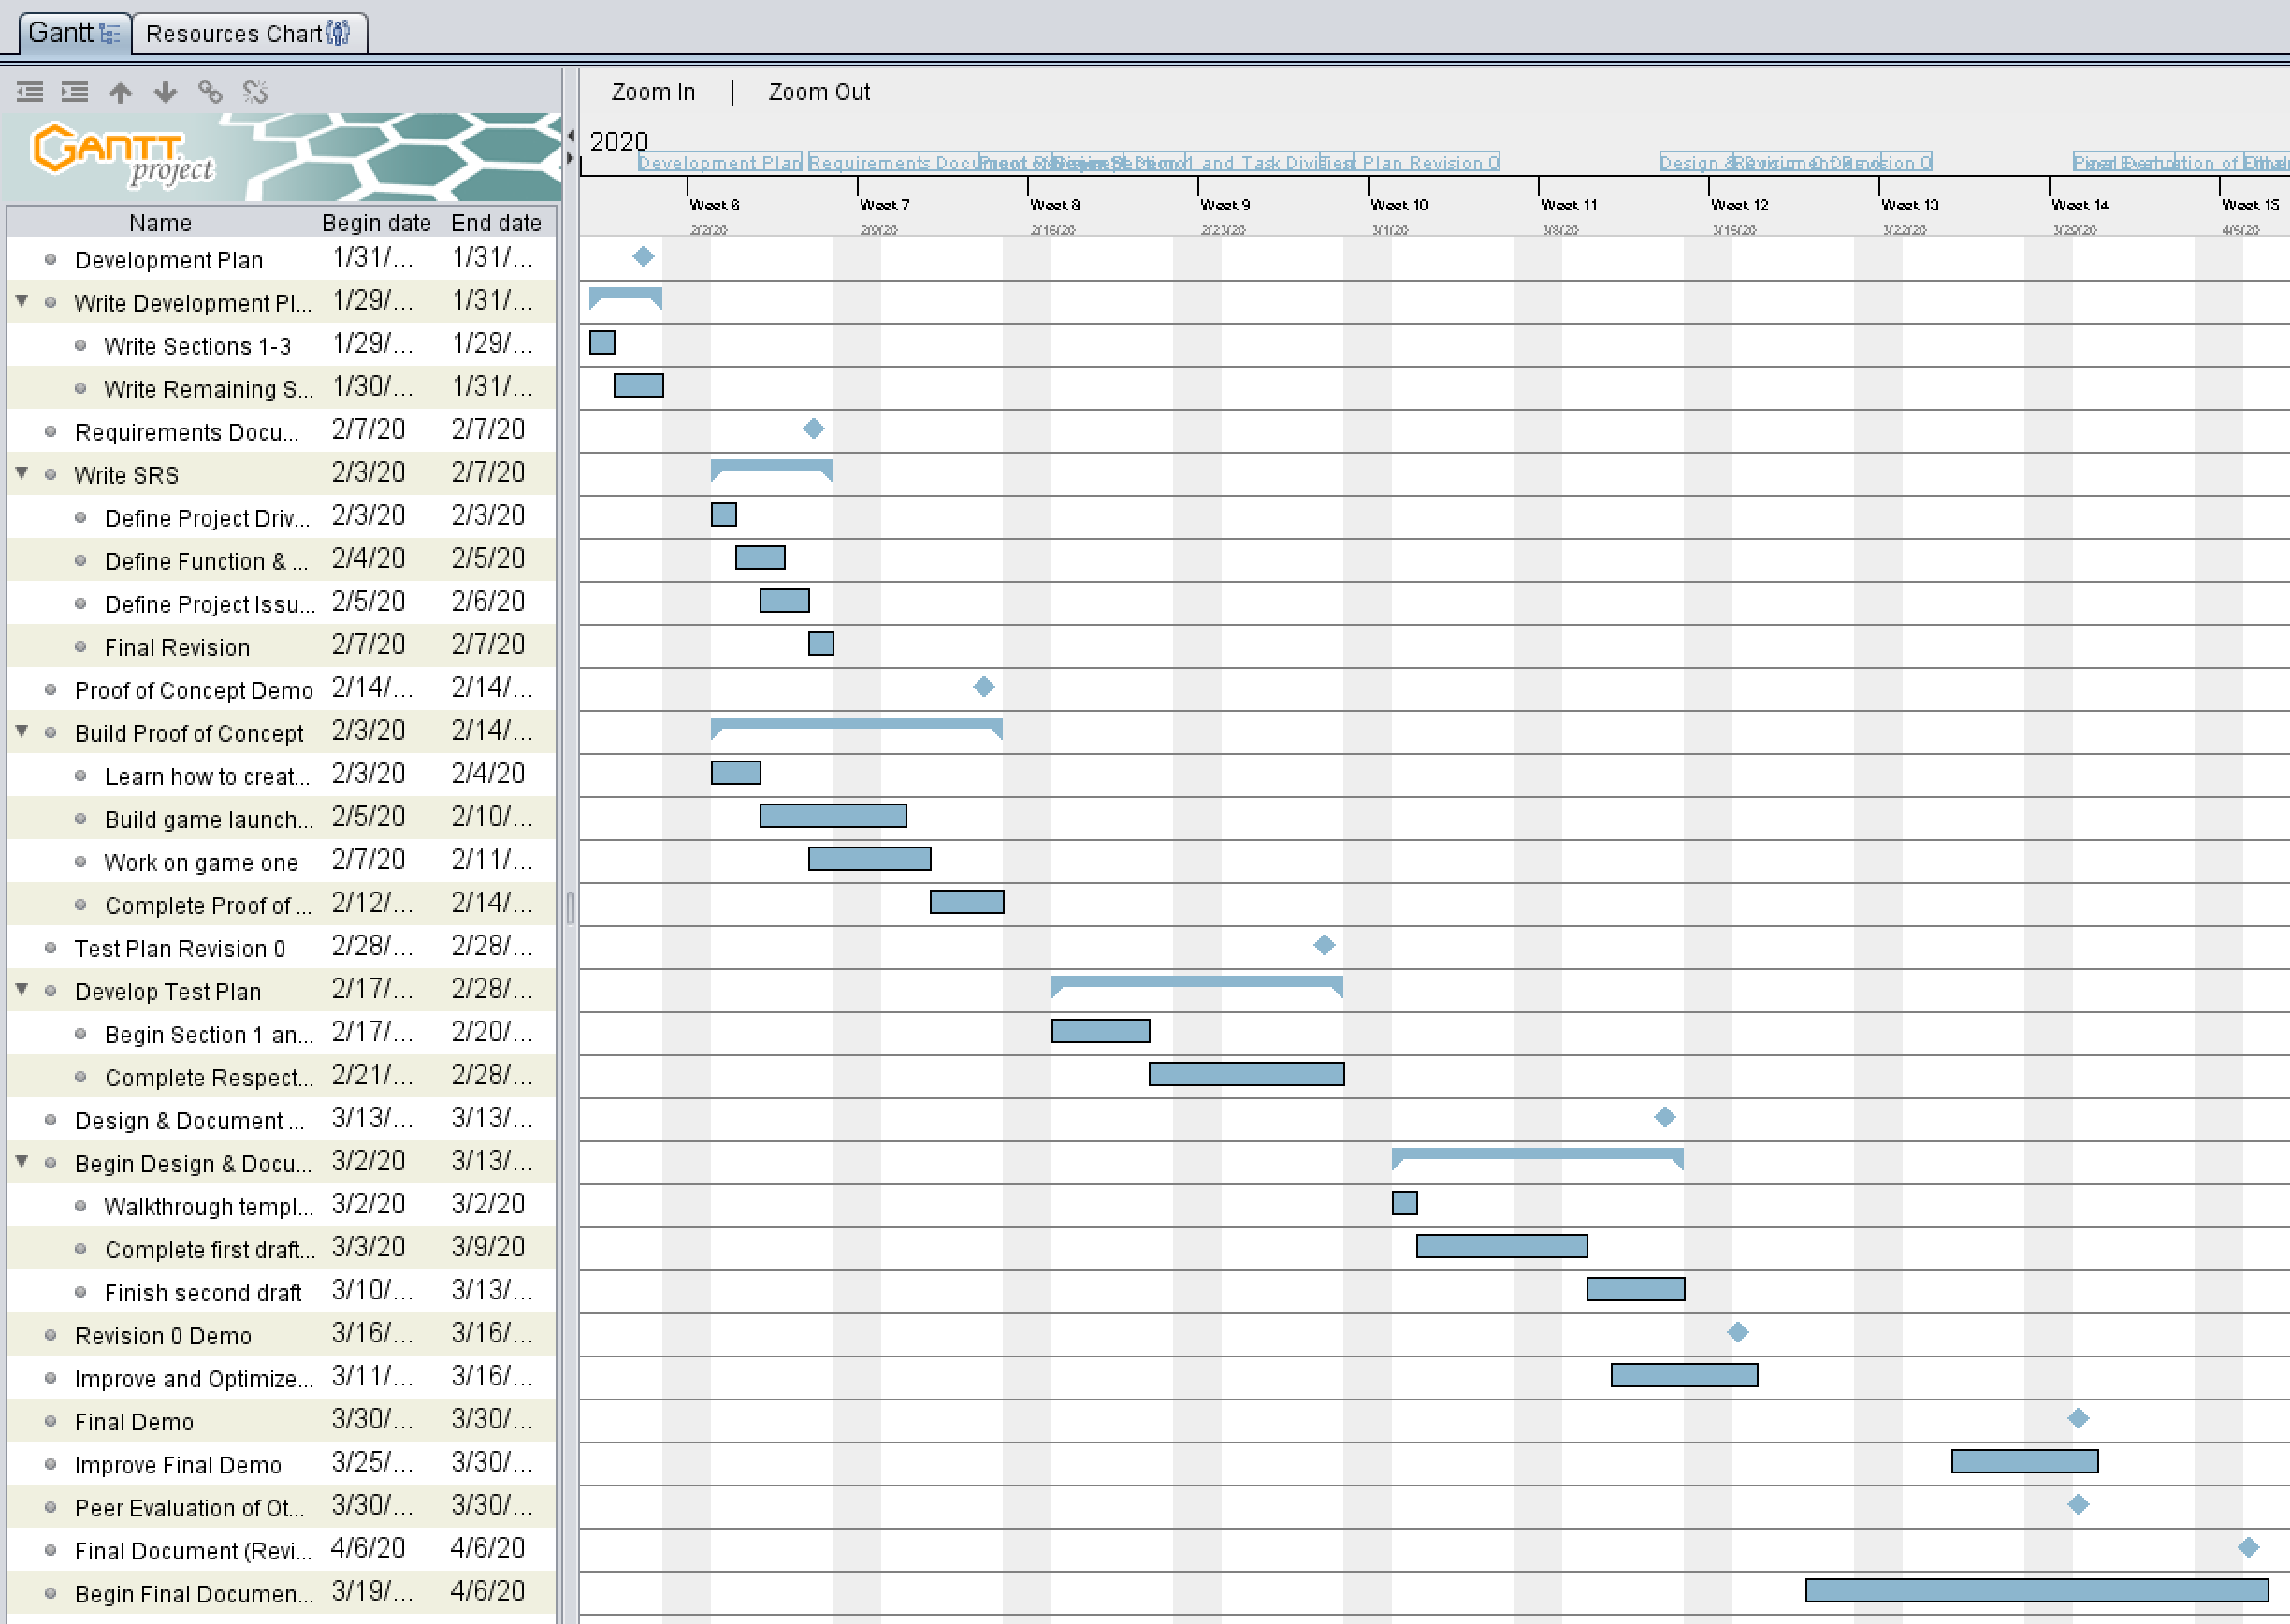
\includegraphics[width=14cm]{TestPlan/GanttRev2.png}\\
\\
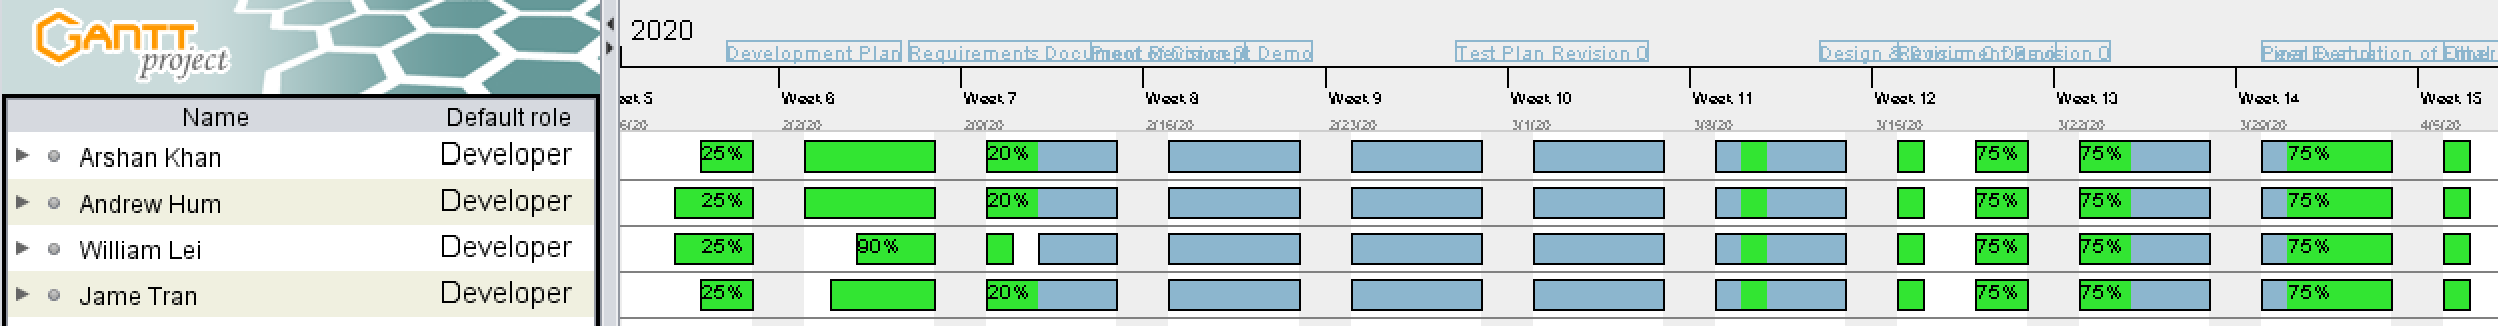
\includegraphics[width=14cm]{TestPlan/GanttRevB2.png}

\section{System Test Description}
	
\subsection{Tests for Functional Requirements}

\subsubsection{General Navigation}

\begin{enumerate}

\item{FR-N-1\\}
Type: FDM\\
Initial State: Main Screen\\
Input: User clicks on Leaderboard\\
Output: Leaderboard opens and is displayed on the screen.\\
How test will be performed: The application will be opened and the user will manually provide inputs to the software and observes for the output of the software on the screen.\\

\item{FR-N-2\\}
Type: FDM\\
Initial State: Main Screen\\
Input: User clicks on Maze\\
Output: The mini-game Maze opens and is displayed on the screen.\\
How test will be performed: The application will be opened and the user will manually provide inputs to the software and observes for the output of the software on the screen.\\

\item{FR-N-3\\}
Type: FDM\\
Initial State: Main Screen\\
Input: User clicks on Flappy\\
Output: The mini-game Flappy opens and is displayed on the screen.\\
How test will be performed: The application will be opened and the user will manually provide inputs to the software and observes for the output of the software on the screen.\\

\item{FR-N-4\\}
Type: FDM\\
Initial State: Main Screen\\
Input: User clicks on Pong\\
Output: The mini-game Pong opens and is displayed on the screen.\\
How test will be performed: The application will be opened and the user will manually provide inputs to the software and observes for the output of the software on the screen.\\

\item{FR-N-5\\}
Type: FDM\\
Initial State: Main Screen\\
Input: User clicks on close button\\
Output: The software will be terminated.\\
How test will be performed: The application will be opened and the user will manually provide inputs to the software and observes for the output of the software on the screen.\\

\item{FR-N-6\\}
Type: FDM\\
Initial State: Leaderboard Screen\\
Input: User clicks on Maze\\
Output: The leaderboard screen will display the leaderboard for Maze.\\
How test will be performed: The application will be opened and the user will manually provide inputs to the software and observes for the output of the software on the screen.\\

\item{FR-N-7\\}
Type: FDM\\
Initial State: Leaderboard Screen\\
Input: User clicks on Flappy\\
Output: The leaderboard screen will display the leaderboard for Flappy.\\
How test will be performed: The application will be opened and the user will manually provide inputs to the software and observes for the output of the software on the screen.\\

\item{FR-N-8\\}
Type: FDM\\
Initial State: Maze - Menu Screen\\
Input: User clicks on Help\\
Output: The screen will display the instructions for how to play the mini-game.\\
How test will be performed: The application will be opened and the user will manually provide inputs to the software and observes for the output of the software on the screen.\\

\item{FR-N-9\\}
Type: FDM\\
Initial State: Flappy - Menu Screen\\
Input: User clicks on Help\\
Output: The screen will display the instructions for how to play the mini-game.\\
How test will be performed: The application will be opened and the user will manually provide inputs to the software and observes for the output of the software on the screen.\\

\item{FR-N-10\\}
Type: FDM\\
Initial State: Pong - Menu Screen\\
Input: User clicks on Help\\
Output: The screen will display the instructions for how to play the mini-game.\\
How test will be performed: The application will be opened and the user will manually provide inputs to the software and observes for the output of the software on the screen.\\

\item{FR-N-11\\}
Type: FDM\\
Initial State: Maze - Menu Screen\\
Input: User clicks on Leaderboard\\
Output: The leaderboard of the mini-game opens and is displayed on the screen.\\
How test will be performed: The application will be opened and the user will manually provide inputs to the software and observes for the output of the software on the screen.\\

\item{FR-N-12\\}
Type: FDM\\
Initial State: Flappy - Menu Screen\\
Input: User clicks on Leaderboard\\
Output: The leaderboard of the mini-game opens and is displayed on the screen.\\
How test will be performed: The application will be opened and the user will manually provide inputs to the software and observes for the output of the software on the screen.\\

\item{FR-N-13\\}
Type: FDM\\
Initial State: Maze - Menu Screen\\
Input: User clicks on Back\\
Output: The Main Screen opens and is displayed on the screen.\\
How test will be performed: The application will be opened and the user will manually provide inputs to the software and observes for the output of the software on the screen.\\

\item{FR-N-14\\}
Type: FDM\\
Initial State: Flappy - Menu Screen\\
Input: User clicks on Back\\
Output: The Main Screen opens and is displayed on the screen.\\
How test will be performed: The application will be opened and the user will manually provide inputs to the software and observes for the output of the software on the screen.\\

\item{FR-N-15\\}
Type: FDM\\
Initial State: Pong - Menu Screen\\
Input: User clicks on Back\\
Output: The Main Screen opens and is displayed on the screen.\\
How test will be performed: The application will be opened and the user will manually provide inputs to the software and observes for the output of the software on the screen.\\

\end{enumerate}

\subsubsection{Mini-Game - Maze}

\begin{enumerate}

\item{FR-MGM-1\\}
Type: FDM\\
Initial State: Maze - Menu Screen\\
Input: User clicks on a difficulty level\\
Output: A maze will be displayed on the screen.\\
How test will be performed: The application will be opened and the user will manually provide inputs to the software and observes for the output of the software on the screen.\\

\item{FR-MGM-2\\}
Type: FDM\\
Initial State: Maze - Game Screen\\
Input: User clicks on home\\
Output: Menu screen of Maze will be displayed on the screen.\\
How test will be performed: The application will be opened and the user will manually provide inputs to the software and observes for the output of the software on the screen.\\

\item{FR-MGM-3\\}
Type: FDM\\
Initial State: Maze - Menu Screen\\
Input: User clicks on a specific difficulty level, then clicks home, and repeats this for 5 times in total\\
Output: A maze will be displayed on the screen every time the user clicks a difficulty level, and there should be no patterns for when a specific maze will be displayed.\\
How test will be performed: The application will be opened and the user will manually provide inputs to the software and observes for the output of the software on the screen.\\

\item{FR-MGM-4\\}
Type: FDM\\
Initial State: Maze - Game Screen\\
Input: User clicks a movement key\\
Output: The object will move according to the key-movement mapping and the movement will be displayed on the screen.\\
How test will be performed: The application will be opened and the user will manually provide inputs to the software and observes for the output of the software on the screen.\\

\item{FR-MGM-5\\}
Type: FDM\\
Initial State: Maze - Game Screen\\
Input: Object reaches the end of the maze through a movement\\
Output: A score (base on time elapsed) along with high score will be displayed on the end game screen.\\
How test will be performed: The application will be opened and the user will manually provide inputs to the software and observes for the output of the software on the screen.\\

\item{FR-MGM-6\\}
Type: FDM\\
Initial State: Maze - End Game Screen\\
Input: User clicks on Next\\
Output: A maze will be displayed on the screen.\\
How test will be performed: The application will be opened and the user will manually provide inputs to the software and observes for the output of the software on the screen.\\

\item{FR-MGM-7\\}
Type: FDM\\
Initial State: Maze - End Game Screen\\
Input: User clicks on Return\\
Output: The Menu Screen opens and is displayed on the screen.\\
How test will be performed: The application will be opened and the user will manually provide inputs to the software and observes for the output of the software on the screen.\\
    
\end{enumerate}

\subsubsection{Mini-Game - Flappy}

\begin{enumerate}

\item{FR-MGF-1\\}
Type: FDM\\
Initial State: Flappy - Menu Screen\\
Input: User clicks on start\\
Output: The game will be initialized/started and the game screen will be opened and displayed\\
How test will be performed: The application will be opened and the user will manually provide inputs to the software and observes for the output of the software on the screen.\\

\item{FR-MGF-2\\}
Type: FDM\\
Initial State: Flappy - Game Screen\\
Input: User controlling the character to make sure it will not collide with any object\\
Output: There will be randomly generated objects approaching toward the character, and their speed and amount generated will be increased as time elapses.\\
How test will be performed: The application will be opened and the user will manually provide inputs to the software and observes for the output of the software on the screen.\\

\item{FR-MGF-3\\}
Type: FDM\\
Initial State: Flappy - Game Screen\\
Input: User clicks space key for 5 times separated by a short period\\
Output: The character will move up a constant amount every time the space key is being clicked.\\
How test will be performed: The application will be opened and the user will manually provide inputs to the software and observes for the output of the software on the screen.\\

\item{FR-MGF-4\\}
Type: FDM\\
Initial State: Flappy - Game Screen\\
Input: User controls the character to collide with an object\\
Output: A score (base on time elapsed) along with high score will be displayed on the end game screen.\\
How test will be performed: The application will be opened and the user will manually provide inputs to the software and observes for the output of the software on the screen.\\

\item{FR-MGF-5\\}
Type: FDM\\
Initial State: Flappy - End Game Screen\\
Input: User clicks on Restart\\
Output: The game will be initialized/started and the game screen will be opened and displayed.\\
How test will be performed: The application will be opened and the user will manually provide inputs to the software and observes for the output of the software on the screen.\\

\item{FR-MGF-6\\}
Type: FDM\\
Initial State: Flappy - End Game Screen\\
Input: User clicks on Return\\
Output: The Menu Screen opens and is displayed on the screen.\\
How test will be performed: The application will be opened and the user will manually provide inputs to the software and observes for the output of the software on the screen.\\
    
\end{enumerate}

\subsubsection{Mini-Game - Pong}

\begin{enumerate}

\item{FR-MGP-1\\}
Type: FDM\\
Initial State: Pong - Menu Screen\\
Input: User clicks on Single Player\\
Output: The game screen will be opened and displayed and will request the user to input a max score.\\
How test will be performed: The application will be opened and the user will manually provide inputs to the software and observes for the output of the software on the screen.\\

\item{FR-MGP-2\\}
Type: FDM\\
Initial State: Pong - Menu Screen\\
Input: User clicks on Multiplayer\\
Output: The game screen will be opened and displayed and will request the user to input a max score.\\
How test will be performed: The application will be opened and the user will manually provide inputs to the software and observes for the output of the software on the screen.\\

\item{FR-MGF-3\\}
Type: FDM\\
Initial State: Pong - Game Screen (Both single and multiplayer, requesting max score input)\\
Input: User inputs an integer between 1 to 10.\\
Output: The game will be initialized or started.
How test will be performed: The application will be opened and the user will manually provide inputs to the software and observes for the output of the software on the screen.\\

\item{FR-MGP-4\\}
Type: FDM\\
Initial State: Pong - Game Screen (Both single and multiplayer)\\
Input: User clicks a movement key\\
Output: The corresponding paddle will move according to the key-movement mapping and the movement will be displayed on the screen.\\
How test will be performed: The application will be opened and the user will manually provide inputs to the software and observes for the output of the software on the screen.\\

\item{FR-MGP-5\\}
Type: FDM\\
Initial State: Pong - Game Screen (Both single and multiplayer)\\
Input: User control the paddle to hit the ball until the ball reaches the boundary on either side (and did not hit a paddle)\\
Output: The score of the opposite will be increased by 1 and the change will be displayed on the game screen.\\
How test will be performed: The application will be opened and the user will manually provide inputs to the software and observes for the output of the software on the screen.\\

\item{FR-MGF-6\\}
Type: FDM\\
Initial State: Flappy - Game Screen (Both single and multiplayer)\\
Input: User control the paddle to hit the ball until either side reaches the max score\\
Output: The score between the two players will be displayed on the end game screen.\\
How test will be performed: The application will be opened and the user will manually provide inputs to the software and observes for the output of the software on the screen.\\

\item{FR-MGP-7\\}
Type: FDM\\
Initial State: Pong - End Game Screen\\
Input: User clicks on Restart\\
Output: The game will be initialized/started and the game screen will be opened and displayed.\\
How test will be performed: The application will be opened and the user will manually provide inputs to the software and observes for the output of the software on the screen.\\

\item{FR-MGP-8\\}
Type: FDM\\
Initial State: Pong - End Game Screen\\
Input: User clicks on Return\\
Output: The Menu Screen opens and is displayed on the screen.\\
How test will be performed: The application will be opened and the user will manually provide inputs to the software and observes for the output of the software on the screen.\\
    
\end{enumerate}

\subsection{Tests for Nonfunctional Requirements}

\subsubsection{Look and Feel}
	
\begin{enumerate}

\item{NFR-1\\}

Type: FDM
					
Initial State: The program is launched on default settings, with default performance settings on the computer, at the start screen of one of three games (Flappy, Maze, or Pong).
					
Input/Condition: Users will be asked to play the game for 5 minutes.
					
Output/Result: Average FPS displayed by pygame get\_fps() is higher than 30.
					
How test will be performed: A test group of people who have graduated high school or have an equivalent GED will be asked to play the games (Maze, Pong, and Flappy Bird) for a total of 5 minutes. The average FPS will be recorded by using the built-in method get\_fps() in pygame. The majority of the test group must have an average FPS of 30 or above for the test to be considered successful.
					
\item{NFR-2\\}

Type: FDM
					
Initial State: The program is launched on default settings, with default performance settings on the computer, at the start screen of one of three games (Flappy, Maze, or Pong).
					
Input: Users will be asked to play the game for 5 minutes.
					
Output: Users in the test group will be asked to evaluate the existing implementation of the games' visual appeal.
					
How test will be performed: A test group of people who have graduated high school or have an equivalent GED will be asked to play the games (Maze, Pong, and Flappy Bird) for a total of 5 minutes. They will then complete a survey that has a list of criteria related to each games' visual design, with each criterion attached to a Likert scale. The users will be asked to rate the program based on the criteria provided using the scales provided.  The average rating for each criterion will be calculated. The average must be above 3 on each criterion for the test to be considered successful. 

					

\end{enumerate}

\subsubsection{Usability and Humanity}

\begin{enumerate}

\item{NFR-3\\}

Type: FDM
					
Initial State: The program is launched on default settings, with default performance settings on the computer, at the start screen of one of three games (Flappy, Maze, or Pong).
					
Input: Users will be asked to play the game for 5 minutes
					
Output: Users in the test group will be asked to evaluate the existing implementation and intrusiveness of the games' UI.

How test will be performed: A test group of people who have graduated high school or have an equivalent GED will be asked to play the games (Maze, Pong, and Flappy Bird) for a total of 5 minutes. They will then complete a survey that has a list of criteria related to each games' UI design, with each criterion attached to a Likert scale. The users will be asked to rate the program based on the criteria provided using the scales provided.  The average rating for each criterion will be calculated. The average must be above 3 on each criterion for the test to be considered successful. 



\item{NFR-4\\}

Type: FFDM
					
Initial State: The program is launched on default settings, with default performance settings on the computer, at the start screen of one of three games (Flappy, Maze, or Pong).
					
Input: Users will be asked to play the game for 5 minutes.
					
Output: Users in the test group will be asked to evaluate the controls and game-play of the existing implementation of the games.

How test will be performed: A test group of people who have graduated high school or have an equivalent GED will be asked to play the games (Maze, Pong, and Flappy Bird) for a total of 5 minutes. Afterwards, each user will complete a small quiz on the respective game they played, with questions about core game-play mechanics. The quizzes will be marked, and an average score of 80\% on the quizzes is required for success.


\end{enumerate}

\subsection{Performance}
\begin{enumerate}
\item{NFR-5\\}

Type: FDM
					
Initial State: The program is launched on default settings, with default performance settings on the computer. 
					
Input: The user will be asked to launch one of three games (Flappy, Maze, or Pong).
					
Output: The requested action is performed in less than 30 seconds.

How test will be performed: Either a group of users will be asked to perform the task or the task will be iterated multiple times. The average time elapsed between launching the game and the game being fully functional will be recorded. The requested action must be performed under 30 seconds for 80\%  of the times the test is performed.

\item{NFR-6\\}

Type: FDM
					
Initial State: The program is launched on default settings, with default performance settings on the computer, currently playing one of three games (Flappy, Maze, or Pong).
					
Input: The user will be asked to make an input into the game.
					
Output: The game will be updated within a quarter second of user input.

How test will be performed: Either a group of users will be asked to perform the task or the task will be iterated multiple times. The average time elapsed between making an input and the game updating will be recorded. The requested action must be performed within a quarter second for 80\%  of the times the test is performed.
\end{enumerate}

\subsection{Operation and Environmental Requirements}
\begin{enumerate}
\item{NFR-7\\}

Type: FDM
					
Initial State: A computer powered on, without Mini-Arcade currently installed.
					
Input: The user will be asked to install the program.

Output: The majority of users can install the program without outside assistance.

How test will be performed: Either a group of users will be asked to perform the task or the task will be iterated multiple times. The program installation success and the amount of time it took will be recorded. The test is considered successful if 80\% of users can install the program without assistance. This test will be repeated on multiple computers with varying hardware and operating systems
\end{enumerate}

\section{Tests for Proof of Concept}

\subsection{Area of Testing}
		
\paragraph{Since many of the above tests for non-functional requirements also cover issues in the Proof of Concept, these tests will focus on testing external modules}

\begin{enumerate}

\item{PC-1\\}

Type: FDM
					
Initial State: A computer with Python 3 installed, the source code for the projects, and the pyinstaller module installed.
					
Input: The user will create an executable of the source files using pyinstaller.
					
Output: A working executable file will be created.
					
How test will be performed: A sample python file will be used for testing. The user will create an executable using pyinstaller, and run the executable. Success will be counted if the executable program can display game functionality. This test will be repeated across multiple computers.
					
\item{test-id2\\}

Type: FDM
					
Initial State: A computer with VSCode and Python 3 installed.
					
Input: The user will attempt to install the Pygame module
					
Output: The Pygame module will be available for use in VSCode
					
How test will be performed: The user will use Pip to install the Pygame module in a virtual environment. The user will then attempt to import the Pygame module and run a sample program that uses its functionality. If the program can run and display full functionality, the test is a success. This test will be repeated across multiple computers.

\end{enumerate}
	
\section{Unit Testing Plan}

The Pytest library will be used for the unit testing of our project.
		
\subsection{Unit testing of internal functions}

To efficiently use unit-testing for our project, we will use hard-coded, expected, and unexpected, inputs for individual functions and methods. These functions and methods will then provide output, and we will verify that the resulting output is correct or that the program handles the unexpected input correctly. For example, telling the game that the game was won, and the expected output should be the end-game screen. As games are more difficult to completely test with unit tests, we will only test the functions that can be tested by providing an expected and unexpected output with input values relating to a current state or completed event. To cover a wide range of scenarios, the input variables will test both expected output, and reaction to incorrect/unexpected input values. There will be no need for stubs or drivers to test our project. To ensure high-quality coverage, we will be using testing coverage metrics. Our goal is to cover a minimum of 60\% of the project with unit tests alone, derived by the total lines of code in the project divided by the number of lines covered by the test cases.
	
\subsection{Unit testing of output files}	

In-depth testing of the output files using unit testing will be not applicable for our project, and any unit tests to test output files would prove to be not useful and ineffective in both coverage and effective use of time.

\bibliographystyle{plainnat}

\bibliography{SRS}

\newpage

\section{Appendix}

\subsection{Usability Survey Questions}

A set of questions to ask potential system testers would include:
\begin{itemize}
    \item What game did you play first?
    \item What did you think of that game?
    \item How long did you play?
    \item Would you play again?
    \item Did you play any other games?
    \item Was it easy to get started?
    \item How would you improve the experience?
    \item Was the system easy to understand?
    \item Was the system easy to navigate?
\end{itemize}

\end{document}
